\documentclass[a4]{scrreprt}

\usepackage{geometry}
\usepackage{graphicx}
\usepackage{amsmath}
\usepackage{listings}
\usepackage{color}
\usepackage[disable]{todonotes} % draft/disable
\usepackage{longtable, tabu}
\usepackage{needspace}
\usepackage{hyperref}

\geometry{left=2.5cm, right=2cm, top=1.5cm, bottom=1.5cm, includeheadfoot}

\definecolor{mygreen}{RGB}{28,172,0} % color values Red, Green, Blue
\definecolor{mylilas}{RGB}{170,55,241}

\lstset{language=Matlab,%
	%basicstyle=\color{red},
	breaklines=true,%
	morekeywords={matlab2tikz},
	keywordstyle=\color{blue},%
	morekeywords=[2]{1}, keywordstyle=[2]{\color{black}},
	identifierstyle=\color{black},%
	stringstyle=\color{mylilas},
	commentstyle=\color{mygreen},%
	showstringspaces=false,%without this there will be a symbol in the places where there is a space
	numbers=left,%
	numberstyle={\tiny \color{black}},% size of the numbers
	numbersep=9pt, % this defines how far the numbers are from the text
	emph=[1]{for,end,break},emphstyle=[1]\color{red}, %some words to emphasise
	%emph=[2]{word1,word2}, emphstyle=[2]{style},    
}

\setcounter{tocdepth}{4}
\begin{document}
	
\begin{titlepage}
	\centering
	
	\large MATLAB Library Documentation\\[2cm]
		
	\huge\textbf{Multidimensional Time Series Toolbox}\\[1cm]
	
	\begin{figure}[!h]
		\centering
		
\includegraphics[width=3cm]{Media/IALogo.jpg}
	\end{figure}
	
	\vspace{1cm}
	
	\Large Institute for Automation\\[0.3cm]
	
	\normalsize
	Department Product Engineering\\[0.3cm]
	Montanuniversit\"at Leoben\\[2cm]

	\Large Thomas Grandl,\\Roland Ritt\\[2cm]		
	
	\large Version: 1.2\\
	\large \today
	
	\vfill
	
	% Bottom of the page
	\copyright\ \the\year, Institute for Automation, University of Leoben\\
	\url{automation.unileoben.ac.at}\\
	All Rights Reserved
	
\end{titlepage}

\tableofcontents

\chapter{Introduction}
\section{Download}
This toolbox can be downloaded from the IA-GitLab Server.
\begin{itemize}
	\item Web-Url: \url{https://git.unileoben.ac.at/Chair-Of-Automation/IA-toolboxes/mdtsToolbox}
	\item Git-Link: \url{git@git.unileoben.ac.at:Chair-Of-Automation/IA-toolboxes/mdtsToolbox.git}
\end{itemize}

\section{Purpose of this Toolbox}

This toolbox provides tools for handling time series in multi dimensions. It implements a data storage for these time series together with the according metadata. Various functions and methods provide tools for the extraction and extension, as well as the initialization, analysis and manipulation of the data.

\section{Toolbox Structure}

The structure of the toolbox is illustrated in figure \ref{FigToolboxStructure}.

\begin{figure}[htbp]
	\centering
	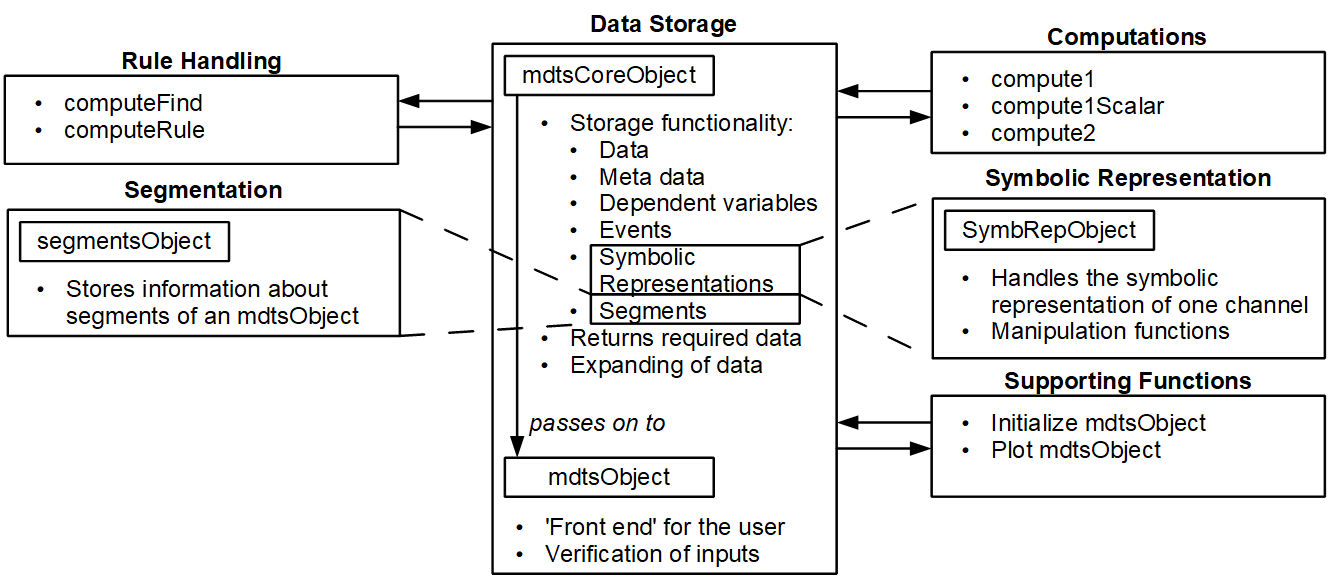
\includegraphics[width=\textwidth]{Media/ToolboxStructure.png}
	\caption{Structure of the toolbox}
	\label{FigToolboxStructure}
\end{figure}

\subsection{Data Storage}
\label{ChpIDDataStorage}

The data storage is implemented as two classes, the \textit{mdtsCoreObject} Class and the \textit{mdtsObject} Class.

The mdtsCoreObject represents the actual data storage. It holds all time series (data) as well as additional information about these series (metadata). It also provides functions to extract specific parts of the data as well as to extend the data set by a new time series. Furthermore, events and symbolic representations of channels can be added to the mdtsCoreObject.

The mdtsObject is a ``wrapper class'' which inherits from the mdtsCoreObject. It represents the interface between the data storage and the user or computational functions, respectively. It has the same functions as the core object. This way it validates the inputs and passes them to the actual functions of the mdtsCoreObject.

The user is expected to only use the mdtsObject, direct usage of the mdtsCoreObject is restricted to internal processes for faster execution!

\subsection{Symbolic Representation}

The data of every channel can be discretized and represented through symbols. Such a symbolic representation is implemented as separate object. If a channel is represented symbolically, a \textit{SymbRepObject} is generated and assigned to this channel. The mdtsCoreObject holds the handles to every available SymbRepObject and the assignment to the according channel. Beside the representation of the data, the SymbRepObject provides a number of functions to analyse and manipulate the symbolic representation of a channel.

\subsection{Computations}

A set of functions is available to execute various computations.

\subsection{Rule Handling}

A set of functions to find specific states within the data and to combine or superpose states with rules.

\subsection{Segmentation}

The data of a mdtsObject can be devided into segments. Such a segment can for example represent the occurrence of certain events. One instance of such a segment is represented by its start time and the duration together with the name of the segment. For example, if a mdtsObject contains data of a certain machine, one segmentation could represent the running times of this machine, where one instance of this segmentation represents the start when the machine is turned on and the time it is running. The segmentation and the \textit{segmentsObject}, respectively, can followingly include multiple of such instances with different start times and durations.

\subsection{Supporting Functions}

Further functions are available to initialize and inspect (plot) the data.

\section{Dependencies}

The mdtsToolbox requires the following IA-toolboxes in the MALTAB-path:

\begin{enumerate}
	\item IAToolboxes/DOPbox: Git-Link \url{git@git.unileoben.ac.at:Chair-Of-Automation/IA-toolboxes/DopBox.git}
	\item IAToolboxes/graphics: Git-Link \url{git@git.unileoben.ac.at:Chair-Of-Automation/IA-toolboxes/graphics.git}
	\item IAToolboxes/general: Git-Link \url{git@git.unileoben.ac.at:Chair-Of-Automation/IA-toolboxes/general.git}
	\item IAToolboxes/figureManager: Git-Link \url{git@git.unileoben.ac.at:Chair-Of-Automation/IA-toolboxes/figureManager.git}
	\item IAToolboxes/summaryTable: Git-Link \url{git@git.unileoben.ac.at:Chair-Of-Automation/IA-toolboxes/summarytable.git}
\end{enumerate}

\chapter{Class and Function Description}

\section{Data Storage}

\subsection{mdtsCoreObject}
\label{ChpDescriptionMdtsCoreObject}

\subsubsection{Properties}

\begin{enumerate}
	\item Core data:
	\begin{enumerate}	
		\item \textbf{time:} n x 1 vector of time stamps. Can be given as datenum, datetime, duration or any arbitrary numerical vector
		\item \textbf{data:} n x m matrix of values
		\item \textbf{tags:} 1 x m vector of series names as strings (character vectors)
		\item \textbf{tsEvents:} Map which holds all events. Keys are event IDs as character vector (string) and values are structs, where value.eventTime represents an array of all time stamps when the event starts and value.eventDuration represents an array of all durations of the event as number of time stamps. Furthermore, the user can add specific data to every event in the field value.userData.
		\item \textbf{symbReps:} Cell array which holds all symbolic representations. The representation of a channel is stored in the cell array as the element with the index according to the channel or tag index. Further descriptions in section \ref{ChpDescriptionSymbRepObject}.	
		\item \textbf{segments:} Variable which holds a segmentsObject, compare section \ref{ChpDescriptionSegmentsObject}.
		\item \textbf{aliasTable:} A table which holds the aliases for tags. The row names are the aliases, and the column \emph{OrigTag} holds the name of the original tag. If you request a tag, it first searches through this table, and after this, it searches in the tags itself.
	\end{enumerate}
	\item Meta data:
	\begin{enumerate}	
		\item \textbf{name:} name of the object/time series
		\item \textbf{who:} creator of the object/time series
		\item \textbf{when:} creation date of the object/time series as string
		\item \textbf{description:} description to the object/time series
		\item \textbf{comment:} comment to the object/time series    
		\item \textbf{units:} units of the tags
		\item \textbf{uniform:} ture if the time steps are spaced uniformly
		\item \textbf{ts:} sampling time
		\item \textbf{isSubset:} true if the object was derived by extraction from another mdtsObject
		
	\end{enumerate}
	\item Dependent data:
	\begin{enumerate}	
		\item \textbf{fs:} sampling frequency
		\item \textbf{timeRelative:} relative time stamps in which the first stamp starts at zero
		\item \textbf{timeDateTime:} time stamps in datetime format
		\item \textbf{timeDateTimeRelative:} relative time stamps in which the first stamp starts at zero in datetime format
		\item \textbf{nChannels:} number of Channels in the mdts-Object (number of Columns)
		\item \textbf{nDataPoints:} number of DataPoints (time-stamps); this is the number of rows
	\end{enumerate}
\end{enumerate}

The structure of these properties within the mdtsCoreObject is illustrated in figure \ref{FigmdtsCoreObjectStructure}.

\begin{figure}[htb]
	\centering
	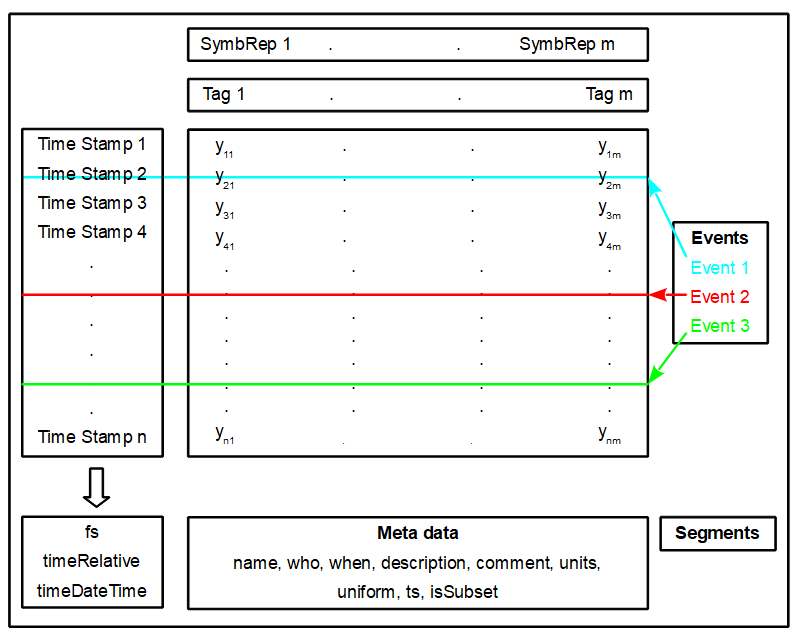
\includegraphics[width=0.8\textwidth]{Media/mdtsCoreObjectStructure.png}
	\caption{Structure of the properties within the mdtsCoreObject}
	\label{FigmdtsCoreObjectStructure}
\end{figure}

\subsubsection{Constructor}

\begin{align*}
\text{obj} = \text{mdtsCoreObject}(&\text{time, }\text{data,  }\text{tags, }\text{units, }\text{ts, }\text{name, }\\&\text{who, }\text{when, }\text{description, }\text{comment, }\text{tsEvents, }\text{symbReps, }\text{segments, }\text{aliasTable})
\end{align*}

Inputs must be given according to the properties of the object.

\subsubsection{Methods}

\begin{enumerate}
\item \textbf{returnObject = getData}\\
	Returns a new object with extracted data from the original object. The following function calls are available:	
	\begin{align*}
		\text{returnObject} =& \text{ getData(tags)}\\
		\text{returnObject} =& \text{ getData(tags, timeInterval)}
	\end{align*}	
	where \textit{tags} is a string which represents the name of the time series or a 1 x m cell array of strings which represent the names of multiple time series and \textit{timeInterval} is a 2 x 1 array of time stamps as datenum which define start and end of the time interval, e.g.
	\begin{lstlisting}[frame=single]
tags = {'Channel1', 'Channel2', 'Channel3'};
timeInterval = [datenum(datetime(2017, 7, 31, 14, 3, 3, 123));
		datenum(datetime(2017, 7, 31, 14, 3, 3, 123 + 5))];
returnObject = originalObject.getData(tags, timeInterval);
	\end{lstlisting}
\item \textbf{dataMat = getRawData}\\
	Returns the data from the mdtsObject as specified in the input parameters. The following function calls are available:
	\begin{align*}
	\text{dataMat} =& \text{ getRawData(tags)}\\
	\text{dataMat} =& \text{ getRawData(tags, timeInterval)}
	\end{align*}	
	where \textit{tags} is a string which represents the name of the time series or a 1 x m cell array of strings which represent the names of multiple time series, \textit{timeInterval} is a 2 x 1 array of time stamps as datenum which define start and end of the time interval and \textit{dataMat} is the extracted matrix from the data of the mdtsObject, e.g.
	\begin{lstlisting}[frame=single]
tags = {'Channel1', 'Channel2', 'Channel3'};
timeInterval = [datenum(datetime(2017, 7, 31, 14, 3, 3, 123));
datenum(datetime(2017, 7, 31, 14, 3, 3, 123 + 5))];
dataMat = originalObject.getRawData(tags, timeInterval);
	\end{lstlisting}
\item \textbf{tagIndices = getTagIndices(tagList)}\\
	Returns indices of the tags given in \textit{tagList}. tagList must be given as string which represents the name of the time series or as 1 x m cell array of strings wich represent the names of multiple time series, e.g.
	\begin{lstlisting}[frame=single]
tagList = {'Channel1', 'Channel2', 'Channel3'};
tagIndices = originalObject.getTagIndices(tagList);
	\end{lstlisting}
\item \textbf{intervalIndices = getIntervalIndices(timeInterval)}\\
	Returns indices of the time interval given in \textit{timeInterval}. timeInterval must be given as 2 x 1 array of time stamps as datenum which define start and end of the time interval, e.g.
	\begin{lstlisting}[frame=single]
timeInterval = [datenum(datetime(2017, 7, 31, 14, 3, 3, 123));
		datenum(datetime(2017, 7, 31, 14, 3, 3, 123 + 5))];
intervalIndices = originalObject.getIntervalindices(timeInterval);
	\end{lstlisting}
\item \textbf{correctTags = checkTags(tagList)}\\
	Checks if the tags given in \textit{tagList} are available within the data set. Returns a boolean which is true when tags are available, otherwise false. tagList must be given as string which represents the name of the time series or as 1 x m cell array of strings which represent the names of multiple time series, e.g.
	\begin{lstlisting}[frame=single]
tagList = {'Channel1', 'Channel2', 'Channel3'};
correctTags = originalObject.checkTags(tagList);
	\end{lstlisting}
\item \textbf{[startDateNum, endDateNum] = startEndOfDate(dateString)}\\
	Returns the first and the last available time stamp of a time span as datenum. The time span must be given in \textit{dateString} as string (see example below). For example, if the data contains one time stamp every day from January 1st, 2015 to December 31st, 2017 and \textit{dateString} is ``2016'', then \textit{startDateNum} is the datenum of January 1st, 2016 and endDateNum is the datenum of December 31st, 2016. Possible values for dateString are given in the following example:
	\begin{lstlisting}[frame=single]
dateString1 = '25-Jul-2017 14:03'; % 14:03:00 to 14:03:59 on 7/25/2017
dateString2 = '25-Jul-2017 2pm'; % 14:00:00 to 14:59:59 on 7/25/2017
dateString3 = '25-Jul-2017'; % 00:00:00 to 24:59:59 on 7/25/2017
dateString4 = 'Aug-2017'; % 00:00:00 on 8/1/2017 to 24:59:59 on 8/31/2017

[startDateNum1, endDateNum1] = originalObject.startEndOfDate(dateString1);
[startDateNum2, endDateNum2] = originalObject.startEndOfDate(dateString2);
[startDateNum3, endDateNum3] = originalObject.startEndOfDate(dateString3);
[startDateNum4, endDateNum4] = originalObject.startEndOfDate(dateString4);
	\end{lstlisting}
\item \textbf{obj = expandDataSet(addData, addTags)}\\
	Expands the data set of the object by the (multiple) time series given in \textit{addData} and assigns these new series the tags given in \textit{addTags}. addData must be given as n x m matrix of data values and addTags as string which represents the name of the time series or as 1 x m cell array of strings which represent the names of multiple time series, e.g.
	\begin{lstlisting}[frame=single]
addTags1 = 'Channel1';
addData1 = [3;
	    4;
	    5];
addTags2 = {'Channel1', 'Channel2'};
addData2 = [3, 6;
	    4, 7;
	    5, 8;
	    6, 9];
addTags3 = {'Channel1', 'Channel2', 'Channel3'};
addData3 = [3, 6, 10;
	    4, 7, 11;
	    5, 8, 12;
	    6, 9, 13];
	    7, 10, 14];
	    
originalObject1 = originalObject1.expandDataSet(addData1,addTags1);
originalObject2 = originalObject2.expandDataSet(addData2,addTags2);
originalObject3 = originalObject3.expandDataSet(addData3,addTags3);
originalObject4 = originalObject4.expandDataSet(addData4,addTags4);
	\end{lstlisting}
\item \textbf{Direct Indexing}\\
It is also possible to extract a part from the mdtsCoreObject as
\begin{align*}
\text{newmdtsCoreObject} = \text{ originalmdtsCoreObject}(i : j, k : l)
\end{align*}
where $i, j$ are the time indices and $k, l$ are the tag indices, e.g.
\begin{lstlisting}[frame=single]
newObject = originalObject(2 : 4, 1 : 3); % time stamps 2 - 4, tags 1 - 3
newObject = originalObject(1 : 4, 2 : 3); % time stamps 1 - 4, tags 2 - 3
newObject = originalObject(4, 1 : 3); % time stamp 4, tags 1 - 3
newObject = originalObject(2 : 5, 2); % time stamps 2 - 5, tags 3
\end{lstlisting}

\item \textbf{obj = addEvent(eventID, eventTime, eventDuration)}\\
	Adds an event to \textit{tsEvents} such that $tsEvents(key) = value$ with the key \textit{eventID} and a struct as value with the two entries \textit{eventTime} as value.eventTime, as well as \textit{eventDuration} as value.eventDuration.

\item \textbf{obj = addSymbRepToChannel(channelNumber, symbObj)}\\
	Adds the symbRepObject \textit{symbObj} to \textit{symbReps} as element with index \textit{channelNumber}.
	
\item \textbf{obj = addSymbRepToAllChannels(symbObj, keepExistentSymbReps)}\\
Adds the symbRepObject \textit{symbObj} to all elements of \textit{symbReps}. If \textit{keepExistentSymbReps} is true, already existent symbRepObjects within \textit{symbReps} will be preserved, if set to false, all elements in \textit{symbReps} will be overwritten.

\item \textbf{obj = addSegments(segmentsObj)}\\
Stores the segmentsObject \textit{segmentsObj} in the \textit{segments} property of the mdtsObject.

\item \textbf{obj = addSegmentsToAllChannels(segmentsObj, keepExistentSegReps)}\\
Assigns the segmentsObject \textit{segmentsObj} to all channels in the \textit{segments} property of the mdtsObject. If \textit{keepExistentSegReps} is true, already existent segmentsObjs within \textit{segments} will be preserved, if set to false, all elements in \textit{segments} will be overwritten.

\item \textbf{obj = addSegmentsToChannels(segmentsObj, channelNumber)}\\
Assigns the segmentsObject \textit{segmentsObj} to  \textit{segments} the property of the mdtsObject for only the given channelNumber(s).

\end{enumerate}

\subsubsection{Methods (Protected)}
These functions can only be called within the class or a subclass.

\begin{enumerate}
	
	\item \textbf{obj = keepRowsOfData(intervalIndices)}\\
	Delete all data (rows) of time stamps which are not given in \textit{intervalIndices}. \textit{intervalIndices} are the numeric indices of the rows to be kept.
	
	\item \textbf{obj = keepTagsOfData(tagsIndices)}\\
	Delete all data (columns) oftags which are not given in \textit{tagsIndices}. \textit{tagsIndices} are the numeric indices of the columns to be kept.
	
	\item \textbf{extractRowsOfSymbReps(intervalIndices)}\\
	Extract all symbols and druations from the symbRepObjects of all channels, according to the input \textit{intervalIndices}. \textit{intervalIndices} are the numeric indices of the rows to be kept. The symbReps are overwritten with the trimmed version.
	
	\item \textbf{extractRowsOfSegsReps(intervalIndices)}\\
	Extract all segments and druations from the segmentsObject of all channels, according to the input \textit{intervalIndices}. \textit{intervalIndices} are the numeric indices of the rows to be kept. The segments are overwritten with the trimmed version.
	
	\item \textbf{extractIntervalOfEvents(intervalIndices)}\\
	Extract all events from the eventsStruct of all channels, according to the input \textit{intervalIndices}. \textit{intervalIndices} are the numeric indices of the rows to be kept. The events are overwritten with the trimmed version. ATTENTION: This method is not yet implemented.
	
	\item \textbf{tags = alias2tag(tags)}\\
	returns the tag names which is assigned to the \textit{aliases}. \textit{tags} are the original tag names which are assigned to the aliases.
\end{enumerate}

\subsection{mdtsObject}

As mentioned in section \ref{ChpIDDataStorage}, the mdtsObject inherits from the mdtsCoreObject. Thus, this object has the same properties available as the mdtsCoreObject in addition to the properties stated here.

\subsubsection{Properties}

\begin{enumerate}
	
	\item Internal data:\\
	Note: Internal data is only for the usage in one object and for the communication between different objects. These are no properties the user should deal with!
	
		\begin{enumerate}
			
			\item \textbf{timeType:} Scalar which holds the information about the original time format which was used to initialize the object. Possible variants are datetime, duration, datenum or other numerical representations. This property will be set by the constructor of the mdtsObject automatically, according to the type of the given time vector.
			\begin{enumerate}
				\item \textbf{timeType == 0, timeType == 1}: the time was given as numeric values; and are treated like this $\rightarrow$ no datetime representation is used for plotting etc.
				\item \textbf{timeType == 2}: the time was given as datetime values; and are treated like this in plotting
				\item \textbf{timeType == 3}: the time was given as duration values; and are treated like this in plotting
			\end{enumerate}		
		\end{enumerate}
	
	\item Dependent data:	
		\begin{enumerate}	
			\item \textbf{timeInFormat:} Time stamps of the object in the format according to the original format which was used to initialize the object. 
		\end{enumerate}
	
\end{enumerate}

\subsubsection{Constructor}

\begin{align*}
\text{obj} = \text{mdtsObject}(\text{time, }\text{data,  }\text{tags, }\text{varargin})
\end{align*}

where \textit{time}, \textit{data} and \textit{tags} are required inputs and \textit{varargin} represents all optional inputs. Required inputs must be given according to the porperties of the mdtsCoreObject (compare section \ref{ChpDescriptionMdtsCoreObject}). Optional inputs can be given as tuples. The available optional inputs are summarized in table \ref{TblMdtsConstructorInputs}.

\begin{table}[htbp]
	\centering
	\caption{Available optional inputs for mdtsObject constructor}
	\begin{tabular}{ | c | l | l |}
		\hline
		Input & Description & Default Values \\ \hline \hline
		`units' & Units of the corresponding tags & `-' \\ \hline
		`ts' & Sampling time & [] \\ \hline
		`name' & Name of the data set & `Time Series' \\ \hline
		`who' & Creator of the object & `Author' \\ \hline
		`when' & Date when the object was created & `Now' \\ \hline
		`description' & Description to the object & `No description available' \\ \hline
		`comment' & Comment to the object & `No comment available' \\ \hline
		`tsEvents' & Events within the data & Empty map \\ \hline
		`symbReps' & Symbolic representations & Empty cell array \\ \hline
		`segments' & Segments of the mdtsObject & Empty cell array \\ \hline
		`aliasTable' & aliases for the tags & Emty table with column `OrigTag'  \\ \hline
	\end{tabular}
	\label{TblMdtsConstructorInputs}
\end{table}

\subsubsection{Methods}

\begin{enumerate}
	
\item \textbf{returnObject = getData}\\
	Validates the inputs and passes these inputs to the \textit{getData} function of the mdtsCoreObject, compare section \ref{ChpDescriptionMdtsCoreObject}.
	
\item \textbf{dataMat = getRawData}\\
Validates the inputs and passes these inputs to the \textit{getRawData} function of the mdtsCoreObject, compare section \ref{ChpDescriptionMdtsCoreObject}.
	
\item \textbf{tagIndices = getTagIndices(tagList)}\\
	Validates the inputs in \textit{tagList} and passes them to the \textit{getTagIndices} function of the mdtsCoreObject, compare section \ref{ChpDescriptionMdtsCoreObject}.
	
\item \textbf{intervalIndices = getIntervalIndices(timeInterval)}\\
	Checks if the given time interval lies within the bounds of the time stamps of the object and passes them to the \textit{getIntervalIndices} function of the mdtsCoreObject, compare section \ref{ChpDescriptionMdtsCoreObject}.
	
\item \textbf{obj = expandDataSet(addData, addTags)}\\
	Validates the inputs and passes them to the \textit{expandDataSet} function of the mdtsCoreObject, compare section \ref{ChpDescriptionMdtsCoreObject}.
	
\item \textbf{Direct Indexing}\\
Furthermore its possible to extract data from the mdtsObject as 
\begin{align*}
\text{newObject} = \text{ originalObject}(i : j, k : l)
\end{align*}
where $i, j$ are the time indices and $k, l$ are the tag indices, e.g.
\begin{lstlisting}[frame=single]
newObject = originalObject(2 : 4, 1 : 3); % time stamps 2 - 4, tags 1 - 3
newObject = originalObject(1 : 4, 2 : 3); % time stamps 1 - 4, tags 2 - 3
newObject = originalObject(4, 1 : 3); % time stamp 4, tags 1 - 3
newObject = originalObject(2 : 5, 2); % time stamps 2 - 5, tag 2
newObject = originalObject(:, 2); % all time stamps , tag 2
newObject = originalObject(2 : 5, :); % time stamps 2-5 , all tags
\end{lstlisting}
additional tags/alias names can be used for indexing
\begin{lstlisting}[frame=single]
newObject = originalObject(:,{'tag1', 'tag3'}); % all data extracted for channels named with 'tag1' and 'tag3'
newObject = originalObject(:,{'tag1', 'alias3'}); % all data extracted for channels named with 'tag1' and the alias 'alias3'
\end{lstlisting}

In case a datetime vector was used for generating the mdtsObject, datetimes  can be used for row-indexing

\begin{lstlisting}[frame=single]
newObject = originalObject({datetime(2019,8,12), datetime(2019,9,12) },:); % all data extracted between 2019-08-12 and 2019-09-12 (including start and end date),
\end{lstlisting}

\item \textbf{obj = addEvent(eventID, eventTime, eventDuration)}\\
Validates if \textit{eventID} is a character vector (string), \textit{eventTime} is an array of time stamps available in \textit{time} and \textit{eventDuration} is an array of integers or durations and of the same size as \textit{eventTime}. Valid values will be passed to the \textit{addEvent} function of the mdtsCoreObject, compare section \ref{ChpDescriptionMdtsCoreObject}.

\item \textbf{obj = addSymbRepToChannel(channelNumber, symbObj)}\\
Validates if \textit{symbObj} is a symbRepObject and \textit{channelNumber} is numeric and passes valid parameters to the \textit{addSymbRepToChannel} function of the mdtsCoreObject, compare section \ref{ChpDescriptionMdtsCoreObject}.

\item \textbf{obj = addSymbRepToAllChannels(symbObj, varargin)}\\
Validates if \textit{symbObj} is a symbRepObject and passes valid parameters to the \textit{addSymbRepToAllChannels} function of the mdtsCoreObject, compare section \ref{ChpDescriptionMdtsCoreObject}. Optional parameter \textit{keepExistentSymbReps} can be passed as logical scalar through a name-value-pair.

\item \textbf{obj = addSegmentsToAllChannels(segmentsObj, varargin)}\\
Validates if \textit{segmentsObj} is a segmentsObj and \textit{nTimestamps} in \textit{segmentsObj} is the same as the number of elements in \textit{time} of the mdtsObject and passes valid parameters to the \textit{addSegmentsToAllChannels} function of the mdtsCoreObject, compare section \ref{ChpDescriptionMdtsCoreObject}.

\item \textbf{obj = addSegments(segmentsObj)}\\
Validates if \textit{segmentsObj} is a segmentsObj and \textit{nTimestamps} in \textit{segmentsObj} is the same as the number of elements in \textit{time} of the mdtsObject and passes valid parameters to the \textit{addSegments} function of the mdtsCoreObject, compare section \ref{ChpDescriptionMdtsCoreObject}.

\item \textbf{obj = addSegmentsToChannels(segmentsObj, channelNames)}\\
Validates if \textit{segmentsObj} is a segmentsObj and \textit{nTimestamps} in \textit{segmentsObj} is the same as the number of elements in \textit{time} of the mdtsObject and passes valid parameters to the \textit{addSegmentsToChannels} function of the mdtsCoreObject, compare section \ref{ChpDescriptionMdtsCoreObject}. \textit{channelNames} is a cell array of tags or aliases to which the segments should be assigned.

\item \textbf{timeDateNum = convert2Datenum(timeInput)}\\
Converts a time in \textit{timeInput} from datetime or duration to datenum (if \textit{timeInput} is given as datenum, then \textit{timeDateNum = timeInput}).

\item \textbf{bValid = isValidAliasTable(tIn)}\\
This function checks, if a table \textit{tIn} is a valid aliasTable with respect to the tags of the mdtsObject \textit{obj.tags}. It checks if the table has exactly one column \textit{OrigTag} and if the entries in this column can be found in \textit{obj.tags}.

\item \textbf{isTagList = isTag(tags)}\\
This function checks, if the given \textit{tags} can be found within the taglist of the object or within the aliasTable. It returns a logical array of the same size as \textit{isTagList} indicating if a tag is can be found and used for indexing.

\item \textbf{obj =  setAliasTable(tIn)}\\
This function assignes a new aliasTable \textit{tIn} to the mdtsObject. All aliases defined before are deleted in this manner.

\item \textbf{isInList = isAlias( tags)}\\
This function checks if the given \textit{tags} are aliases defined in the aliasTable of the instance. A logical array \textit{isInList} of the same size as \textit{tags} is returned, indicating which tags are aliases.

\item \textbf{obj = addAliases(aliases, tags)}\\
This function adds new aliases to the aliasTable. aliases is a list of new names which can be used to index the mdtsObject. Tags is the original tag name which is used to index the mdtsObject.

\item \textbf{obj = markRangeOnAxes\_givenIndex(axes\_in, startInds, stopInds, colorSpec, varargin)}\\
This function marks a given range as a semitransparent patch. It forwards the input parameters to the Static-Method \textit{markRangeOnAxes\_givenIndexStatic} and takes the time values from the mdtsObject.
(see \textit{mdtsOjbect} \ref{sssec:mdtsObj:MethodsStatic} \nameref{sssec:mdtsObj:MethodsStatic})

\item \textbf{arrayOfmdtsObjects = extractSegments(segmentTag, tagName, varargin)}\\
This functions extracts segments from the segments  structure and returns them as mdtsObjects (cell array of mdtsObjects \textit{arrayOfmdtsObjects}). \textit{segmentTag} is the name of the Segment which should be extracted. \textit{tagName} is the name of the channel to which the \textit{segmentTag} is assigned. \textit{frameLength} (optional key-value pair; default value = 0) defining how much data points should be additionally returned to the beginning and at the end of each segment.




\item \textbf{summaryTable = getSummaryTable}\\
This functions returns a \textit{summaryTable} for the given mdtsObject. Therefore, the according toolbox (\textit{summaryTable}) need to be on the matlab path.

\item \textbf{[axesH, fM, ph] = plot(varargin)}\\
This functions plots the mdtsObject (stacked plot with Events and Symbolic Time Series represented as Semi-Transparent patches). The optional input arguments (key-value pairs) are:
	\begin{enumerate}
		\item \textbf{Size}: the size (height, width) of the plot im centimeters. Default Value: [8.8cm, 11.7cm] 
		\item \textbf{FontSize}: the font Size in pt used for figure. Default value: 10pt
		\item \textbf{plotSymbolName}: boolean flag indicating if the symbol should be plotted on the semi transparent patches (if a SymbolicRepresentation is defined). Default: false
		\item \textbf{plotSymbolDuration}: boolean flag indicating if the symbol duration should be plotted on the semi transparent patches (if a SymbolicRepresentation is defined). Default: false
		\item \textbf{plotSymbolNameMinLengthRelative}: the minimum length of a symbolic representation to show the symbol name and duration defined as a relative value of the entire length of the time series. Default: 0.05; this can be used to avoid clattering of the plot in case of short symbols.
		\item \textbf{figureH}: a handle to a figure which should be used for plotting. Default: a new figure is created with \textit{figureGen} of the graphics-toolbox.
		\item \textbf{additional key-value pairs}: are forwarded to the plotMulti function of the graphics-toolbox.
	\end{enumerate}
returned are:
	\begin{enumerate}
		\item \textbf{axesH}: the handles to the axes
		\item \textbf{fM}: the figureManager used on the figure to handle large data sets (figureManager-toolbox)
		\item \textbf{ph}: the handles to the plotted timeseries (handles to the line objects).
	\end{enumerate}

\item \textbf{ph = plotEventsOnAxes(axesIn)}\\
This function plots the event assigned to the mdtsObject on given axes  (\textit{axesIn} as a dashed line at the point of occurence. \textit{axesIn} are the axes on which the Events should be plotted. \textit{ph} are the handles to the event-lines (line-objects).
	
\item \textbf{[axesOut, fM, ph] = plotmdtsObject(inputObject, varargin)}\\
is a deprecated method which currently forwards \textit{varargin} to the \textit{plot} function of \textit{mdtsObject}.

\item \textbf{[axesOut, fM, ph] = plotSegments(segmentTag, varargin)}\\
Will be deprecated in future. This function generates a new plot of the multidimensional time series where the assigned segments are marked as semi-transparent patches.
The input arguments are:
	\begin{enumerate}
		\item \textbf{segmentTag}: the name of the segment which should be plotted
		\item \textbf{Size}: optional; the size (height, width) of the plot im centimeters. Default Value: [8.8cm, 11.7cm] 
		\item \textbf{FontSize}: optional; the font Size in pt used for figure. Default value: 10pt
		\item \textbf{other key-value pairs}: are forwarded to the plotMulti function of the graphics-toolbox.
	\end{enumerate}
returned are:
	\begin{enumerate}
		\item \textbf{axesH}: the handles to the axes
		\item \textbf{fM}: the figureManager used on the figure to handle large data sets (figureManager-toolbox)
		\item \textbf{ph}: the handles to the plotted segments (handles to the patches objects objects).
	\end{enumerate}

\item \textbf{ph = plotSegmentsOnAxes(axesIn, segmentTag, varargin)}\\
Will be deprecated in future. This function plots the assigned segments on the given \textit{axesIn} as semi-transparent patches.
The input arguments are:
	\begin{enumerate}
		\item \textbf{axesIn}: the axes on which the segments should be plotted
		\item \textbf{segmentTag}: the name of the segment which should be plotted
		\item \textbf{other key-value pairs}: are forwarded to segmentsObject.plotOnAxes.
	\end{enumerate}
returned are:
	\begin{enumerate}
		\item \textbf{ph}: the handles to the plotted segments (handles to the patches objects objects).
	\end{enumerate}

\end{enumerate}

\subsubsection{Methods (Static)}
\label{sssec:mdtsObj:MethodsStatic}
\begin{enumerate}
	
	\item \textbf{bValid = isValidAliasTableTags(tIn, tags)}\\
	This function checks, if a table \textit{tIn} is a valid aliasTable with respect to the given \textit{tags}. It checks if the table has exactly one column \textit{OrigTag} and if the entries in this column can be found in \textit{tags}.
	
	\item \textbf{isInList = isTagWithinTagList(tags, taglist)}\\
	This function checks, if the \textit{tags} (cell array) are within the cell-array  \textit{taglist}. It returns a boolean list \textit{isInList} with the same size as \textit{tags} where the value 1 indicates if the tags are available in the given \textit{taglist}.
	
	\item \textbf{bValid = isTagWithinAliasTable(tags, aliasTab)}\\
	This function checks, if the \textit{tags} (cell array) are within the alias table  \textit{aliasTab}. It returns a boolean list with the same size as \textit{tags} where the value 1 indicates if the tags are available in the given \textit{aliasTab}.
	
	\item \textbf{[pa, tHandleAll] = markRangeOnAxes\_givenIndexStatic(xVals, axes\_in, startInds, stopInds, colorSpec, varargin)}\\
	This function marks a given range as a semitransparent patch. \textit{xVals} is a vector of the xValues used to plot the patches. \text{axes\_in} are the axes, on which the patches should be places. \textit{startInds} and \textit{stopInds} are arrays of the same size containing the indexes to \textit{xVals} where the patches should start and end. \textit{colorSpec} are the color specification for the patch. Optional the key-value pair \textit{textToShow} and a string or cell array of strings of the text which should be shown within the patches. Additional all other key-value pairs are passed on to the \text{fill} command of Matlab. Returned are the handles to the patches and the handles to the text objects.
	
	
\end{enumerate}

\section{Symbolic Representation (Class Defintion)}
\label{ChpSymbolicRepresentation}

\subsection{SymbRepObject (Class Defintion)}
\label{ChpDescriptionSymbRepObject}

\subsubsection{Properties}
\begin{enumerate}
	\item Core Properties:
		\begin{enumerate}
			\item \textbf{symbols:} Complete data of the according channel as sequence of symbols in a n x 1 categorical array. Repetitive symbols are merged to one symbol and the number of repretitions is stored in 'durations' (e.g. three repetitions \{'a', 'a', 'a'\} of the symbol 'a' will be merged to one symbol 'a' with a duration of spanning all three symbols and repetition value is set to 3).
			\item \textbf{durations:} Number of timestamps (datapoints, span of datapoints) of every symbol as n x 1 array. $durations(i)$ represents the number of repetitions of the symbol $symbols(i)$. The sum of this array correlates with the number of time stamps (datapoints) in the channel data.
			\item \textbf{name:} A string (char) of the name of the Symbolic Representation. Can be set with the function \textit{setName}.
			\item \textbf{repetitions:} an array, which contains the number of repetitions of the symbol. Initially, this is set to duration. After merge, this is updated.
		\end{enumerate}
	\item Dependent Properties:
		\begin{enumerate}
			\item \textbf{symbolDurations:} The sum of all durations of the set of unique categories. The duration of all (unique) symbols (categories) are summed up.
			\item \textbf{startInds:} returns a list of the start indices of each symbol (categorie).
			\item \textbf{stoptInds:} returns a list of the stop indices of each symbol (categorie).
			\item \textbf{nSyms:} returns the number of elements in the symbols-array.
		\end{enumerate}
	
	
\end{enumerate}



\subsubsection{Constructor}

\begin{align*}
\text{obj} = \text{SymbRepObject}(\text{durations, }\text{symbols})
\end{align*}

\textit{symbols} must be given as categorical, \textit{durations} must be given as numeric vector of the same dimension as \textit{symbols}.

\subsubsection{Methods}

\begin{enumerate}
	\item \textbf{[startInds, stopInds] = SymbObj.compressedInds2UncompressedInds(indsCompressed)}\\
		Converts given Compressed Indices to uncompressed startIndices and stopIndices. 
		The input arguments are:
		\begin{enumerate}
			\item \textbf{indsCompressed}: a list of indices of the compressed symbolic time series.
		\end{enumerate}
		returned are:
		\begin{enumerate}
			\item \textbf{startInds}: start indices of the requested indices with respect to the  uncompressed series
			\item \textbf{stopInds}: stop indices of the requested indices with respect to the uncompressed series.
		\end{enumerate}
	
	\item \textbf{SymbObj = SymbObj.compressSymbols(listOfSymbolsToCheck)}\\
		This methods of the SymbRepObject finds run-length of the same symbol and replaced it with a single symbol. Additionally, the durations and repetitions are updated by summing up.
		The input arguments are:
		\begin{enumerate}
			\item \textbf{listOfSymbolsToCheck}: A cell array of symbols to be checked and updated. By default all different symbols in the symbolic time series are checked.
		\end{enumerate}
		returned are:
		\begin{enumerate}
			\item \textbf{SymbObj}: a version of the updated SymbRepObject
		\end{enumerate}
	
	\item \textbf{[startInds, durations, compressedStartInds, compressedStopInds] = SymbObj.findSequence(symbSequence)}\\
		Find the start indices, durations, compressed start indices and compressed stop indices of a symbolic sequence.
		%   sequence
		The input arguments are:
		\begin{enumerate}
			\item \textbf{symbSequence}: Sequence (cell array) of symbols, which is to be found within the compressed symbolic time series. Must be given as one dimensional cell an arbitrary number of elements.
		\end{enumerate}
		returned are:
		\begin{enumerate}
			\item \textbf{startInds}: index in the original uncompressed time series where the sequences  start.
			\item \textbf{durations}: the number of samples in the original uncompressed time series the  sequence lasts.
			\item \textbf{compressedStartInds}: the indices where the symbSequence starts in the  compressed symbolic representation
			\item \textbf{compressedEndInds}: the indices  where the symbSequence stops in the  compressed symbolic representation
		\end{enumerate}
	
	
	\item \textbf{[startInds, durations, repetitions] = SymbObj.findSymbol(symbol)}\\
		Returns all indices of the first element of repetitive \textit{symbol} in \textit{symbRepVec} together with the according durations and repetitions, e.g.
		\begin{verbatim}
		>> symbols = categorical({'a'; 'b'; 'a'; 'b'; 'a'});
		>> durations = [2; 4; 3; 5; 2];
		>> symbolicObject = SymbRepObject(durations, symbols);
		>> [startInds, durations] = symbolicObject.findSymbol('a')
		
		startInds =
		
		1
		7
		15	
		
		durations =
		
		2
		3
		2
		\end{verbatim}
		
		The input arguments are:
		\begin{enumerate}
			\item \textbf{symbol}: the symbol to be found within the instance (char)
		\end{enumerate}
		returned are:
		\begin{enumerate}
			\item \textbf{startInds}: the start indices of the occurrances of the symbol within the symbolic representation. The indices are with respect to the datapoints and not to the compressed symbolic structure.
			\item \textbf{durations}: the durations of the occurrances of the symbol within the symbolic representation.
			\item \textbf{repetitions}: the repetitions of the occurrances of the symbol within the symbolic representation.
		\end{enumerate}
	
	\item \textbf{symbInd = SymbObj.findSymbolVec(symbol)}\\
		Returns a boolean array of the size of \textit{symbRepVec} with ``true'' elements on all positions of \textit{symbol}. The result is with respect to the uncompressed symbolic sequence, e.g.
		\begin{verbatim}
		>> symbols = categorical({'a'; 'b'; 'c'});
		>> durations = [2; 3; 1];
		>> symbolicObject = SymbRepObject(durations, symbols);
		>> symbInd = symbolicObject.findSymbolVec('a')
		
		symbInd =
		
		6x1 logical array
		
		1
		1
		0
		0
		0
		0
		\end{verbatim}
		
		The input arguments are:
		\begin{enumerate}
			\item \textbf{symbol}: the symbol to be found within the instance (char)
		\end{enumerate}
		returned are:
		\begin{enumerate}
			\item \textbf{symbInd}:Boolean array indicating on which positions the symbol is contained in the uncompressed symbolic representation. The index can be used for indexing the underlaying time series
		\end{enumerate}
	
	\item \textbf{[allSymbRepObjects, imageMatrix, compressionData, evalRecord] = \\SymbObj.genHierarchicalCompounding(varargin)}\\
		This function is under development. It performs hierarchical compounding on the given SymbObj. Therefore, word pairs, which occur often are compounded to a new word. This is done iteratively.
	
				The input arguments are:
		\begin{enumerate}
			\item \textbf{maxLevel}: (optional key-value) integer defining the maximum number of levels to be calculated.
		\end{enumerate}
		returned are:
		\begin{enumerate}
			\item \textbf{allSymbRepObjects}: Array of SymbRepObjects. Array(i) is the i-th level of hierarchicalCompounding
			\item \textbf{imageMatrix}: Matrix which contains in each row the categorie of each datapoint (symbol) for one level. This can be used to plot the hierarchical development.
			\item \textbf{compressionData}: A struct with information for each level, eg. number of Symbols, number of categories, number of merged Symbols and symbol reduction rate.
			\item \textbf{evalRecord}: A table which contains all steps performed during the hierarchical compounding
		\end{enumerate}

	\item \textbf{[allSymbRepObjects, imageMatrix, compressionData, evalRecord] = \\SymbObj.genHierarchicalCompounding2(SymbObjFunStrg, varargin)}\\
		This function is under development. It is an updated version of \textit{genHierarchicalCompounding}. It performs hierarchical compounding on the given SymbObj. Therefore, word pairs, which occur often are compounded to a new word. This is done iteratively.
	
		The input arguments are:
		\begin{enumerate}
			\item \textbf{SymbObjFunStrg}: name (string) of a function of the SymbRepObject to be used to calculate the symbols to be merged. Currently the following functions are possible:  genLengthWeightedMatrix, genSymbMarkov, genWeightedMatrixChangedLength
			\item \textbf{maxLevel}: (optional key-value) integer defining the maximum number of levels to be calculated.
		\end{enumerate}
		returned are:
		\begin{enumerate}
			\item \textbf{allSymbRepObjects}: Array of SymbRepObjects. Array(i) is the i-th level of hierarchicalCompounding
			\item \textbf{imageMatrix}: Matrix which contains in each row the category of each datapoint (symbol) for one level. This can be used to plot the hierarchical development.
			\item \textbf{compressionData}: A struct with information for each level, eg. number of Symbols, number of categories, number of merged Symbols and symbol reduction rate.
			\item \textbf{evalRecord}: A table which contains all steps performed during the hierarchical compounding
		\end{enumerate}
	
	\item \textbf{[occurenceM, markovM, sumLength1M, sumLength2M] = \\ SymbObj.genLengthWeightedMatrix(varargin)}\\
		\textit{Only for development purposes!} Generate a markov type  matrix for all symbolic combinations with weighted length difference (if the length of symbols to be merged are similar, they are weighted more, this minimizes the problem that a small symbol effects large parts of the symbolic time series). This function can also be used in the method \textit{genHierarchicalCompounding2}.
		The input arguments are:
		\begin{enumerate}
			\item \textbf{Absolute}: (optonal key-value pair) Set to true if result shall represent the  absolute number of transitions from one state to another, set to false (default) if matrix shall represent transition  probabilities
		\end{enumerate}
		returned are:
		\begin{enumerate}
			\item \textbf{occurenceM}: matrix, which counts the occurrences of symbol $i$ is followed by symbol $j$ in the entry \textit{occurenceM(j,i)}  with the weighting included.
			\item \textbf{markovM}:  matrix containing a value for the probability of symbol $i$ is followed by symbol $j$ with the weighting included.
			\item \textbf{sumLength1M}: a matrix containing in the entry $(i,j)$ the overall length of symbol $i$ in the merged sequences of symbol $i-j$.
			\item \textbf{sumLength2M}: a matrix containing in the entry $(i,j)$ the overall length of symbol $j$ in the merged sequences of symbol $i-j$.
		\end{enumerate}
	
	
	\item \textbf{[occurenceM, markovM] = SymbObj.genSymbMarkov(varargin)}\\
		\textit{Only for development purposes!} Generates a markov matrix for the transition from any symbol to any other symbol.
		The following input arguments are available:
		\begin{enumerate}
			\item \textbf{Absolute}: (optonal key-value pair) Set to true if result shall represent the  absolute number of transitions from one state to another, set to false (default) if matrix shall represent transition  probabilities
		\end{enumerate}
			returned are:
		\begin{enumerate}
			\item \textbf{occurenceM}: matrix, which counts the occurrences of symbol $i$ is followed by symbol $j$ in the entry \textit{occurenceM(j,i)}
			\item \textbf{markovM}:  matrix containing a value for the probability of symbol $i$ is followed by symbol $j$. It is the (column) normalized version of occurenceM.
		\end{enumerate}


	\item \textbf{symbCounts3D =  SymbObj.genTrigramMatrix}\\
		\textit{Only for development purposes!} Generate a 3d counting matrix for all sequences of 3 symbols in a row.
		Returned are:
		\begin{enumerate}
			\item \textbf{symbCounts3D}: matrix, which counts the occurrences of symbol $i$ is followed by symbol $j$ and $k$ in the entry \textit{occurenceM(i,j,k)}
		\end{enumerate}


	\item \textbf{[occurenceM, markovM, sumLength1M, sumLength2M, lengthSyms] =\\ SymbObj.genWeightedMatrixChangedLength(varargin)}\\
		\textit{Only for development purposes!} Generate a markov matrix for all symbolic
		 combinations with weighted change of length. This minimizes the problem, that large portion of the symbolic time series get changed.
		 This function can also be used in the method \textit{genHierarchicalCompounding2}.
		 The input arguments are:
		 \begin{enumerate}
		 	\item \textbf{Absolute}: (optonal key-value pair) Set to true if result shall represent the  absolute number of transitions from one state to another, set to false (default) if matrix shall represent transition  probabilities.
		 \end{enumerate}
		 returned are:
		 \begin{enumerate}
		 	\item \textbf{occurenceM}: matrix, which counts the occurrences of symbol $i$ is followed by symbol $j$ in the entry \textit{occurenceM(j,i)}  with the weighting included.
		 	\item \textbf{markovM}:  matrix containing a value for the probability of symbol $i$ is followed by symbol $j$ weighted by length to be changed.
		 	\item \textbf{sumLength1M}: a matrix containing in the entry $(i,j)$ the overall length of symbol $i$ in the merged sequences of symbol $i-j$.
		 	\item \textbf{sumLength2M}: a matrix containing in the entry $(i,j)$ the overall length of symbol $j$ in the merged sequences of symbol $i-j$.
		 	\item \textbf{lengthSyms}: a v containing  the overall length of each symbol. This is the same as SymbObj.symbolDurations.
		 \end{enumerate}
	 
	\item \textbf{startIndUncompressed = SymbObj.getStartInd(obj, indSymbCompressed)}\\
		given the index of a symbol from the compressed return the start index of the uncompressed sequence.
		The input arguments are:
		\begin{enumerate}
			\item \textbf{indSymbCompressed}: the index of the symbol(s) of the  compressed symbol series.
		\end{enumerate}
		returned are:
		\begin{enumerate}
			\item \textbf{startIndUncompressed}:  the start index (indices) of the uncompressed series.	
		\end{enumerate}
	
	\item \textbf{newSymbObj = SymbObj.getTimeInterval(obj, intervalIndices)}\\
		This returns a snipped of the time series object, given numerical indices of the uncompressed series.
		The input arguments are:
		\begin{enumerate}
			\item \textbf{intervalIndices}: an array containing the start and end index of the snipped to be extracted. The indices are with  respect to the uncompressed series.
		\end{enumerate}
		returned are:
		\begin{enumerate}
			\item \textbf{newSymbObj}:  instance of SymbRepObj which contains only the interval to be requested.
		\end{enumerate}
	
	\item \textbf{[pa, tHandleAll] = SymbObj.markSymbSequenceOnAxes(xVals, axes\_in, SymbSequence, colorSpec, varargin)}\\
		\textit{This function is under development. It works together with the stand-alone function markRangeOnAxes\_givenIndexStatic of the mdtsObject class.}
		The function marks a Symbol sequence as semi-transparent patch on a given axes.
		The input arguments are:
		\begin{enumerate}
			\item \textbf{xVals}: The abscissae values used for plotting. These values and the start and stop indices of the symbolic sequence are used to define the start end end of the patch.
			\item \textbf{axes\_in}:  The axes on which the symbolic sequence should be plotted. Currently it can not handle cell-arrays of axes.
			\item \textbf{SymbSequence}: The sequence of symbols (given as cellarray of strings or chars) which should be marked.
			\item \textbf{colorSpec}: A color specification for the patch (either a valid color name or abbreviation, or a rgb color vector).
			\item \textbf{bShowText}: (optional key-value pair) A boolean flag indicating if the symbol should be plotted as text within the patch. Default value: true.
		\end{enumerate}
		returned are:
		\begin{enumerate}
			\item \textbf{pa}:  A list of patches handles.
			\item \textbf{tHandleAll}:  A list of text handles.
		\end{enumerate}
	
	\item \textbf{SymbObj = SymbObj.mergeSequence(symbSequence, varargin)}\\
		Merges all occurences of a given sequence of symbols within the SymbRepObject.
		The input arguments are:
		\begin{enumerate}
			\item \textbf{symbSequence}: Sequence which is supposed to be merged to one new symbol (categorical). Must be given as one dimensional cell array of strings with an arbitrary number of 	elements.
				\item \textbf{bAllowOverlapping}:  (optional key-value pair, default: false) A boolean flag indicating if overlapping sequences are seen as one occurence. Given a symbolic time series 'ababababa' with durations = [1,1,1,1,1,1,1,1,1] and repetitions = [1,1,1,1,1,1,1,1,1] and merge the sequence 'aba'$\rightarrow$ with the new name 'c': if the flag is set to false, the result would be 'cbcba' with durations = [3,1,3,1,1] and repetitions = [1,1,1,1,1]. If the flag is set to true it would result in the symbolic series 'c' with durations = [9], repetitions = [4].
			\item \textbf{newSymbol}: (optional key-value pair, default: 'concatenation of symbSequence')  A string (char) which should replace the found symbSequence.
			\item \textbf{bCompress}: (optional key-value pair, default: true) A boolean flag,  indicating if SymbObj.compressSymbols should be called after merging the sequences. Given a symbolic sequence 'ababab' and the sequence  to be merged 'ab'$\rightarrow$'c': if bCompress=true the resulting symbolic  sequence would be 'c'. If bCompress=false the resulting symbolic  sequence would be 'ccc'.
		\end{enumerate}
		returned are:
		\begin{enumerate}
			\item \textbf{SymbRepObject}:  Instance of SymbRepObject with merged symbolic  representation.
		\end{enumerate}
	
	
	\item \textbf{SymbObj = SymbObj.mergeSymbols(symbolsToMerge, newSymbol, varargin)}\\
		Merges all \textit{symbolsToMerge} symbols (given as cell array of strings) to one new \textit{newSymbol}.
		The input arguments are:
		\begin{enumerate}
			\item \textbf{symbolsToMerge}: Symbols existent in the symbolic representation,  which have to be merged. Input given as cell array of strings.
			\item \textbf{newSymbol}:  New symbol name for the merged symbol sequence, given as  string
			\item \textbf{varargin}: other key-value pairs are passed forward to SymbRepObject.mergeSequence.
		\end{enumerate}
		returned are:
		\begin{enumerate}
			\item \textbf{SymbObj}:  Original object (SymbRepObject) with merged symbols.
		\end{enumerate}
	
	
	\item \textbf{ [paAll, tHandleAll] = SymbObj.plotOnAxes(axes\_in,  varargin)}\\
		Plots an instance of a SymbRepObject on given axes.
		The input arguments are:
		\begin{enumerate}
			\item \textbf{axes\_in}: the axes, on which the symbolic representation should be  plotted;
			\item \textbf{xTime}:  (optional key-value pair, if not given, take the x values of the first line in the axes) the original time axes where the SymbRepObject refers to;
			\item \textbf{plotSymbolName}: (optional key-value, default: false)a boolean indicating if the Symbol name should be shown in the plot;
			\item \textbf{plotSymbolDuration}: optional key-value, default: false )a boolean indicating if the Symbol duration should be shown in the plot;
			\item \textbf{plotSymbolNameMinLength}: (optional key-value, default: 0) an integer, symbols with a length less than  this value are not annotated with symbol name and/or duration;
			\item \textbf{colorDismiss}: (optional key-value, default: no color) a color string or color triplet which should not be in the colors used for shading the plots.
			\item \textbf{additional inputs}: additional key-value pairs are forwarded to the matlab fill function.
		\end{enumerate}
		returned are:
		\begin{enumerate}
			\item \textbf{paAll}:  an array containing the handles to the patches.
			\item \textbf{tHandleAll}:  array containing the handles to the annotations texts.
		\end{enumerate}
	
	\item \textbf{SymbObj = SymbObj.removeShortSymbols(varargin)}\\
		Removes short symbols (symbols with a small duration). The duration of the short symbol is distributed to the enclosing symbols. Multiple successive short symbols will be treated as one short symbol and the sum of the durations will be distributed to the enclosing symbols. The following arguments are available:
		\begin{enumerate}
			\item \textbf{shortSymbolLength: } Definition of a short symbol. All symbols with a length smaller or equal to \textit{shortSymbolLength} will be removed or splitted, respecitvely. Default is 1.
			\item \textbf{maxNumberShortSymbols: } If the number of a sequence of multiple successive short symbols exceeds \textit{maxNumberShortSymbols}, the sequence of these symbols will not be split, but merged to one larger symbol without any label ('$<$undefined$>$' in Matlab). Default is 5.
			\item \textbf{maxShortSymbolSequenceLength: } If the sum of all durations of multiple successive short symbols exceeds \textit{maxShortSymbolSequenceLength}, the sequence of these symbols will not be splitted, but merged to one larger symbol without any label ('$<$undefined$>$' in Matlab). Default is 10.
			\item \textbf{SplittingMode: } Name-Value-Pair. Defines how the duration of short symbols is distributed. Available options: 
			\begin{enumerate}
				\item \textbf{'equal':} durations will be distributed 1 : 1 to the enclosing symbols
				\item \textbf{'weighted':} durations will be distributed due to the length of the two enclosing symbols
			\end{enumerate}
			Default is 'equal'.	
		\end{enumerate}
		
		\textbf{Note:} If a sequence does not exceed the limits in \textit{maxNumberShortSymbols} or \textit{maxShortSymbolSequenceLength} but contains an unlabelled symbol ('$<$undefined$>$' in Matlab), this symbol will be treated as normal symbol and the complete sequence will be distributed to the enclosing symbols.
		
		Example:
		
		\begin{verbatim}
		>> symbols = categorical({'a'; 'b'; 'c'; 'd'; 'e';...
		>> 'f'; 'g'; 'h'; 'i'; 'j'});
		>> durations = [4; 3; 4; 2; 2; 12; 2; 1; 2; 6];
		>> symbolicObject = SymbRepObject(durations, symbols);
		>> symbolicObject = symbolicObject.removeShortSymbols('shortSymbolLength',...
		>> 3, 'maxNumberShortSymbols', 4, 'maxShortSymbolSequenceLength', 4,...
		>> 'SplittingMode', 'weighted');
		>> symbolicObject.symbols
		
		ans = 
		
		5x1 categorical array
		
		a 
		c 
		f 
		<undefined> 
		j 
		
		>> symbolicObject.durations
		
		ans =
		
		6
		6
		15
		5
		6
		\end{verbatim}
			
			
	\item \textbf{SymbObj = SymbObj.removeSymbolsGivenCompressedIndes(indsRemove, varargin)}\\
			Removes symbols defined in indsRemove. The duration of the deleted symbol is distributed to the enclosing symbols. Multiple successive deleted symbols will be treated as one symbol and the sum of the durations will be distributed to the enclosing symbols.
			The following input arguments are available:
			\begin{enumerate}
				\item \textbf{indsRemove: } Indices of the symbols to be removed
				\item \textbf{shortSymbolLength: } Definition of a short symbol. All symbols with a length smaller or equal to \textit{shortSymbolLength} will be removed or splitted, respecitvely. Default is 1.
				\item \textbf{maxNumberShortSymbols: } If the number of a sequence of multiple successive short symbols exceeds \textit{maxNumberShortSymbols}, the sequence of these symbols will not be split, but merged to one larger symbol without any label ('$<$undefined$>$' in Matlab). Default is 5.
				\item \textbf{maxShortSymbolSequenceLength: } If the sum of all durations of multiple successive short symbols exceeds \textit{maxShortSymbolSequenceLength}, the sequence of these symbols will not be splitted, but merged to one larger symbol without any label ('$<$undefined$>$' in Matlab). Default is 10.
				\item \textbf{SplittingMode: } Name-Value-Pair. Defines how the duration of short symbols is distributed. Available options: 
				\begin{enumerate}
					\item \textbf{'equal':} durations will be distributed 1 : 1 to the enclosing symbols
					\item \textbf{'weighted':} durations will be distributed due to the length of the two enclosing symbols
				\end{enumerate}
				Default is 'equal'.	
			\end{enumerate}
			
			\textbf{Note:} If a sequence does not exceed the limits in \textit{maxNumberShortSymbols} or \textit{maxShortSymbolSequenceLength} but contains an unlabelled symbol ('$<$undefined$>$' in Matlab), this symbol will be treated as normal symbol and the complete sequence will be distributed to the enclosing symbols.
	
	\item \textbf{SymbObj = SymbObj.renameSymbol(oldSymbol, newSymbol)}\\
		Renames all \textit{oldSymbol} symbols to \textit{newSymbol}.
		
	\item \textbf{SymbObj = SymbObj.setName(name)}\\
		sets a \textit{name} for the SymbRepObject. This corresponds to the property \textit{SymbObj.name}.
	
	\item \textbf{SymbObj = SymbObj.setSymbolsInRange(newSymbol, range)}\\
		Sets all symbols in \textit{symbRepVec} in the range \textit{range} to \textit{newSymbol}, which is given as character array. Range must be given as array of the form [startIndex, endIndex], where \textit{startIndex} represent the index of the first element of the range and \textit{endIndex} represents the last element of the range in the uncompressed symbolic series, e.g.
		\begin{verbatim}
		>> symbols = categorical({'a'; 'b'; 'c'});
		>> durations = [1; 3; 4];
		>> symbolicObject = SymbRepObject(durations, symbols);
		>> symbolicObject = symbolicObject.setSymbolsInRange('x', [4, 6]);
		>> symbolicObject.symbols
		
		ans = 
		
		4x1 categorical array
		
		a 
		b 
		x 
		c 
		
		>> symbolicObject.durations
		
		ans =
		
		1
		2
		3
		2	
		\end{verbatim}
		
	\item \textbf{symbRepVec = SymbObj.symbRepVec}\\
		Returns the uncompressed symbolic representation as vector of the same size as the time stamps. All repetitive symbols are included in this vector, e.g.	
		\begin{verbatim}
		>> symbols = categorical({'a'; 'b'; 'c'});
		>> durations = [2; 4; 3];
		>> symbolicObject = SymbRepObject(durations, symbols);
		>> fullVector = symbolicObject.symbRepVec
		fullVector = 
		
		  9x1 categorical array
		
		     a 
		     a 
		     b 
		     b 
		     b 
		     b 
		     c 
		     c 
		     c 
		\end{verbatim}
		
		
	\item \textbf{obj = mergeSequence(symbSequence)}\\
		Searches for all incidences of \textit{symbSequence} sequences of symbols in \textit{symbols}. Replaces the symbols of such a sequence by one new symbol, which name is assembled of the symbols of this sequence. Original symbols in such a sequence are identified by enclosing '\{\}', new symbols which represent a merged sequence are identified by enclosing '[]'. Merged symbols can be merged again, thus the function is ready for nested use. \textit{symbSequence} must be given as $1 \times 2$ cell array of strings, representing one symbol of the sequence in every element of the cell array. The durations of the replaced symbols are summed over the complete sequence and set as duration of the new symbol.
		Example:
		\begin{verbatim}
		>> symbols = categorical({'a'; 'b'; 'c'; 'a'; 'b'; 'a'; 'b'});
		>> durations = [2; 3; 1; 2; 1; 3; 2];
		>> symbolicObject = SymbRepObject(durations, symbols);
		>> symbolicObject = symbolicObject.mergeSequence({'a'; 'b'});
		>> symbolicObject.symbols
		
		ans = 
		
		  3x1 categorical array
		
		     [{a}{b}] 
		     c 
		     [{a}{b}] 
		
		>> symbolicObject.durations
		
		ans =
		
		     5
		     1
		     8	
		\end{verbatim}
	
	
	
\end{enumerate}

\subsubsection{Methods (Static)}

	\begin{enumerate}
		\item \textbf{markovM = SymbRepObject.occurenceM2markovM(occurenceM)}\\
			Takes a occurenceM and returns a markov type matrix by normalizing each column.
			The input arguments are:
			\begin{enumerate}
				\item \textbf{occurenceM}: a occurance matrix returned from the functions genLengthWeightedMatrix, genSymbMarkov, genWeightedMatrixChangedLength.
			\end{enumerate}
			returned are:
			\begin{enumerate}
				\item \textbf{markovM}:  a matrix which is normalized by each column. (sum of each column = 1). Therefor, this matrix can be used to  calculate the probability of the next symbol, eg.  newSymbolPropability = markovM*currentSymbolProbabilityVec
			\end{enumerate}
		
		\item \textbf{markovMcleared = clearMarkovM(markovM, occurenceM)}\\
			Replaces all entries in the markovM where sum(occurenceM,1) ==1 with a probability of 0 (this would correspond that a symbol occurse only once in a symbolic time series). Otherwise, a single occurrence would have probability of 100  which causes problems when merging symbols.
			The input arguments are:
			\begin{enumerate}
				\item \textbf{markovM}: a markov type matrix, which contains the probability that the symbol i is followed by symbol j in the entry markovM(j,i).
				\item \textbf{occurenceM}: The number of occurances of the word pair symbol i followed by symbol j can be found in entry occurenceM(j,i).
			\end{enumerate}
			returned are:
			\begin{enumerate}
				\item \textbf{markovMcleared}: The 'cleared' markovMatrix. This removes 100\% probabilities from the markov Matrix. Since a single occurrence of one symbol i causes a probability of 	100\% of the sequence symbol (i) + symbol (i+1).  
			\end{enumerate}
		
	\end{enumerate}

\subsection{symbRepChannel}

\subsubsection{Function Signature:}

\begin{center}
	returnObject = symbRepChannel(input, edges, alphabet)
\end{center}

\subsubsection{Purpose}

Generate the symbolic representation of a given channel of an mdtsObject.

\subsubsection{Input Parameters:}

\begin{longtabu} to \textwidth {|c|X|}
	\hline
	\textbf{Parameter} & \textbf{Description} \\ \hline
	\endhead
	input & Input for the computation as struct which holds the handle to the mdtsObject as input.object and the required tag as input.tag \\ \hline
	edges & Array of length(alphabet) + 1, which contains the edges for the quantization \\ \hline
	alphabet & Array containing the symbols to assign to the values \\ \hline
\end{longtabu}

\subsubsection{Return Parameters:}

\begin{longtabu} to \textwidth {|c|X|}
	\hline
	\textbf{Parameter} & \textbf{Description} \\ \hline
	\endhead
	returnObject  &  symbRepObject with the symbolized channel \\ \hline
\end{longtabu}

\subsubsection{Description}

Function to extract the data from the according channel of the mdtsObject specified in \textit{input}, assign every data point of this channel a symbol given in \textit{alphabet} according to the limits given in \textit{edges}.

\subsection{applyMCLA}

\subsubsection{Function Signature:}

\begin{center}
	mclaSymbRepObject = applyMCLA(symbRepObjectsList)
\end{center}

\subsubsection{Purpose}

Merge symbolic representations of different channel to one representation.

\subsubsection{Input Parameters:}

\begin{longtabu} to \textwidth {|c|X|}
	\hline
	\textbf{Parameter} & \textbf{Description} \\ \hline
	\endhead
	symbRepObjectsList & List of all SymbRepObjects, which are supposed to be merged, as cell array \\ \hline
\end{longtabu}

\subsubsection{Return Parameters:}

\begin{longtabu} to \textwidth {|c|X|}
	\hline
	\textbf{Parameter} & \textbf{Description} \\ \hline
	\endhead
	mclaSymbRepObject  &  SymbRepObject with merged symbolic representation \\ \hline
\end{longtabu}

\subsubsection{Description}

Combines the symbols at every time stamp of an arbitrary number of channels to one symbolic representation.

\section{Computations}

\subsection{compute1}
\label{Chpcompute1Fct}

\subsubsection{Function Signature:}

\begin{center}
	output = compute1(matrix, input)
\end{center}

\subsubsection{Purpose}

Execute convolution operation.

\subsubsection{Input Parameters:}

\begin{longtabu} to \textwidth {|c|X|}
	\hline
	\textbf{Parameter} & \textbf{Description} \\ \hline
	\endhead
	matrix & Convolution matrix, dense or sparse, or convolution vector \\ \hline
	input & Input for the computation. This can be given as:
			\begin{enumerate}
				\item Vector: Double vector holding the data
				\item Struct: Struct which holds the handle to the mdtsObject as input.object and the required tag as input.tag 
			\end{enumerate} \\ \hline
\end{longtabu}

\subsubsection{Return Parameters:}

\begin{longtabu} to \textwidth {|c|X|}
	\hline
	\textbf{Parameter} & \textbf{Description} \\ \hline
	\endhead
	output & Result as vector \\ \hline
\end{longtabu}

\subsubsection{Description}

Apply a convolution with the matrix given in \textit{matrix} on the specified input.

\subsection{compute1Scalar}

\subsubsection{Function Signature:}

\begin{center}
	output = compute1Scalar(operator, scalar, input)
\end{center}

\subsubsection{Purpose}

Execute operation on input.

\subsubsection{Input Parameters:}

\begin{longtabu} to \textwidth {|c|X|}
	\hline
	\textbf{Parameter} & \textbf{Description} \\ \hline
	\endhead
	operator & Computation operator. Possible options are:
			   \begin{enumerate}
			   		\item '*': Element wise multiplikation
			   		\item '/': Element wise division
			   		\item '+': Element wise addition
			   		\item '-': Element wise subtraction
			   		\item handle: handle to other function
			   \end{enumerate} \\ \hline
	scalar & Scalar for the operation \\ \hline
	input & Input for the computation. This can be given as:
	\begin{enumerate}
		\item Vector: Double vector holding the data
		\item Struct: Struct which holds the handle to the mdtsObject as input.object and the required tag as input.tag 
	\end{enumerate} \\ \hline
\end{longtabu}

\subsubsection{Return Parameters:}

\begin{longtabu} to \textwidth {|c|X|}
	\hline
	\textbf{Parameter} & \textbf{Description} \\ \hline
	\endhead
	output & Result as vector \\ \hline
\end{longtabu}

\subsubsection{Description}

Apply the operation specified in operator on the input, using the scalar given in scalar.

\subsection{compute2}

\subsubsection{Function Signature:}

\begin{center}
	outputVector = compute2(operator, input1, input2)
\end{center}

\subsubsection{Purpose}

Execute operation with two inputs.

\needspace{10\baselineskip}
\subsubsection{Input Parameters:}

\begin{longtabu} to \textwidth {|c|X|}
	\hline
	\textbf{Parameter} & \textbf{Description} \\ \hline
	\endhead
	operator & Computation operator. Possible options are:
	\begin{enumerate}
		\item '*': Element wise multiplikation
		\item '/': Element wise division
		\item '+': Element wise addition
		\item '-': Element wise subtraction
		\item 'dot': Inner product (dot product) of both vectors
		\item 'outer': Outer product of both vectors
		\item 'xcorr': Cross correlation between both inputs
		\item handle: handle to other function
	\end{enumerate} \\ \hline
	input1, input2 & Inputs for the computation. They can be given as:
	\begin{enumerate}
		\item Vectors: Double vector holding the data
		\item Structs: Struct which holds the handle to the mdtsObject as input.object and the required tag as input.tag 
	\end{enumerate} \\ \hline
\end{longtabu}

\subsubsection{Return Parameters:}

\begin{longtabu} to \textwidth {|c|X|}
	\hline
	\textbf{Parameter} & \textbf{Description} \\ \hline
	\endhead
	outputVector & Result as vector \\ \hline
\end{longtabu}

\subsubsection{Description}

Apply the operation determined by \textit{operator} on the data of both inputs. Return the result vector in the output parameter.

\subsection{isValidInput}

\subsubsection{Function Signature:}

\begin{center}
	inputType = isValidInput(input)
\end{center}

\subsubsection{Purpose}

Validate input parameter

\needspace{10\baselineskip}
\subsubsection{Input Parameters:}

\begin{longtabu} to \textwidth {|c|X|}
	\hline
	\textbf{Parameter} & \textbf{Description} \\ \hline
	\endhead
	input & input parameter, which has to be validated \\ \hline
\end{longtabu}

\subsubsection{Return Parameters:}

\begin{longtabu} to \textwidth {|c|X|}
	\hline
	\textbf{Parameter} & \textbf{Description} \\ \hline
	\endhead
	inputType & type of the input. Possible input types are: 
				\begin{enumerate}
					\item 1: structured input. The input is a struct where input.object holds a reference to the mdtsObject and input.tag is a valid tag of this mdtsObject
					\item 2: n x 1 vector of numeric elements
					\item 0: input is invalid
				\end{enumerate} \\ \hline
\end{longtabu}

\subsubsection{Description}

Checks if the given input is either a struct with a handle to the mdtsObject and a valid tag or a numeric vector. The output refers to one of these two types or to an invalid input.

\subsection{LDOasConv}

\subsubsection{Function Signature:}

\begin{center}
	derVec = LDOasConv(input, varargin)
\end{center}

\subsubsection{Purpose}

Compute local derivative on input

\needspace{10\baselineskip}
\subsubsection{Input Parameters:}

\begin{longtabu} to \textwidth {|c|X|}
	\hline
	\textbf{Parameter} & \textbf{Description} \\ \hline
	\endhead
	input & Input for the computation. This can be given as:
	\begin{enumerate}
		\item Vector: Double vector holding the data
		\item Struct: Struct which holds the handle to the mdtsObject as input.object and the required tag as input.tag 
	\end{enumerate} \\ \hline
	varargin & The following parameters are available:
	\begin{enumerate}
		\item \textbf{ls:} Support length
		\item \textbf{noBfs:} Number of basis functions
		\item \textbf{order:} Order of the derivative. If set to 0, data of the given input will be smoothed without any differentiation
	\end{enumerate} \\ \hline
\end{longtabu}

\subsubsection{Return Parameters:}

\begin{longtabu} to \textwidth {|c|X|}
	\hline
	\textbf{Parameter} & \textbf{Description} \\ \hline
	\endhead
	derVec & Result of the local derivative (or smoothing, respectively) of the given input as vector \\ \hline
\end{longtabu}

\subsubsection{Description}

Generates a derivative matrix, using the \textit{dop} function from the \textit{DOP-Box}. The parameter $m, n$ or $ls, noBfs$, respectively, can be passed as optional arguments. If they omitted, hard coded values in the \textit{LDOasConv} function will be used. The generated matrix is passed to the \textit{compute1} function (section \ref{Chpcompute1Fct}), together with the input.

\textbf{ATTENTION:} If a vector, instead of a struct, is used as input, the step size of the time stamps will be assumed to be 1! 

\subsection{SmoothAsConv}

\subsubsection{Function Signature:}

\begin{center}
	smoothedData = smoothAsConv(input, varargin)
\end{center}

\subsubsection{Purpose}

Smooth the data in input

\needspace{10\baselineskip}
\subsubsection{Input Parameters:}

\begin{longtabu} to \textwidth {|c|X|}
	\hline
	\textbf{Parameter} & \textbf{Description} \\ \hline
	\endhead
	input & Input for the computation. This can be given as:
	\begin{enumerate}
		\item Vector: Double vector holding the data
		\item Struct: Struct which holds the handle to the mdtsObject as input.object and the required tag as input.tag 
	\end{enumerate} \\ \hline
	varargin & The following parameters are available:
	\begin{enumerate}
		\item \textbf{ls:} Support length
		\item \textbf{noBfs:} Number of basis functions
	\end{enumerate} \\ \hline
\end{longtabu}

\subsubsection{Return Parameters:}

\begin{longtabu} to \textwidth {|c|X|}
	\hline
	\textbf{Parameter} & \textbf{Description} \\ \hline
	\endhead
	smoothedData & Result of the smoothing of the given input as vector \\ \hline
\end{longtabu}

\subsubsection{Description}

Smooths the data given in \textit{input} by usage of the \textit{LDOasConv} function with 'order' 0.

\section{Rule Handling}

\subsection{computeFind}

\subsubsection{Function Signature:}

\begin{center}
	conformElements = computeFind(operator, input, value)
\end{center}

\subsubsection{Purpose}

Find all time stamps in a channel which meet a certain condition

\needspace{10\baselineskip}
\subsubsection{Input Parameters:}

\begin{longtabu} to \textwidth {|c|X|}
	\hline
	\textbf{Parameter} & \textbf{Description} \\ \hline
	\endhead
	operator & Condition operator as string. Available options: $>, <, ==, \sim=, >=, <=$ \\ \hline
	input & Input for the computation as struct which holds the handle to the mdtsObject as input.object and the required tag as input.tag \\ \hline
	value & Reference value for the condition \\ \hline
\end{longtabu}

\subsubsection{Return Parameters:}

\begin{longtabu} to \textwidth {|c|X|}
	\hline
	\textbf{Parameter} & \textbf{Description} \\ \hline
	\endhead
	conformElements & Logical array which indicates the elements of \textit{input} which fulfil the condition \\ \hline
\end{longtabu}

\subsubsection{Description}

Finds all elements of \textit{input} which fulfil the condition according to the operator and the value.

\subsection{computeRule}

\subsubsection{Function Signature:}

\begin{center}
	ruleElements = computeRule(operator, conformElements1, conformElements2)
\end{center}

\subsubsection{Purpose}

Combine or superpose two logical vectors according to a specified operator

\needspace{10\baselineskip}
\subsubsection{Input Parameters:}

\begin{longtabu} to \textwidth {|c|X|}
	\hline
	\textbf{Parameter} & \textbf{Description} \\ \hline
	\endhead
	operator & Rule operator as string. Available options: \&, $\vert$ \\ \hline
	conformElements1, conformElements2 & logical arrays which represent a condition applied to a data set \\ \hline
\end{longtabu}

\subsubsection{Return Parameters:}

\begin{longtabu} to \textwidth {|c|X|}
	\hline
	\textbf{Parameter} & \textbf{Description} \\ \hline
	\endhead
	ruleElements & Logical array which indicates the rule conform elements \\ \hline
\end{longtabu}

\subsubsection{Description}

Finds all elements of which apply to the rule according to the operator

\section{Segmentation}

The structure of the \textit{segmentsObject} is illustrated in an example in figure \ref{FigSegmentsObjectStructure}.

\begin{figure}[htbp]
	\centering
	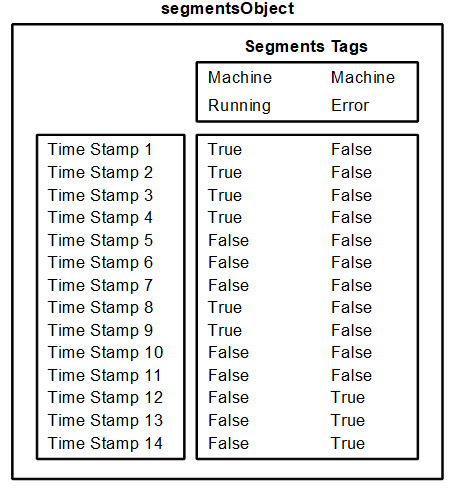
\includegraphics[width=0.5\textwidth]{Media/segmentsObjectStructure.png}
	\caption{Structure of the segmentsObject}
	\label{FigSegmentsObjectStructure}
\end{figure}

This example shows two segments in the segmentsObject: One with the tag label "Machine Running" and one with "Machine Error". The segment "Machine Running" shows two instances of this segment: From time stamp 1 to time stamp 4 and from time stamp 8 to time stamp 9. "Machine Error" shows only one instance from time stamp 12 to time stamp 14. Note that the label in this object refers to the name of the segments - they do not correlate with the tags of the mdtsObject in any way!
To each channel of the mdtsObject one segmentsObject can be assigned.

\subsection{segmentsObject}
\label{ChpDescriptionSegmentsObject}

\subsubsection{Properties}
\begin{enumerate}
	\item Core Data
	\begin{enumerate}
		\item \textbf{nTimestamps:} Total number of time stamps in the segments. Must correlate with the number of time stamps in the data of the according mdtsObject.
		\item \textbf{tags:} Names of the segments as row vector.
		\item \textbf{starts:} Will be renamed in future. Start indices of all instances of the according segment. Stored as cell array (row vector), where every cell contains a column vector representing all start indices of the according segment.
		\item \textbf{durations:} Number of time stamps of every instance of the according segment. Stored as cell array (row vector), where every cell contains a column vector representing all durations of the according segment.
	\end{enumerate}

	\item Dependend Properties
	\begin{enumerate}
		\item \textbf{startInds:} Start indices of all instances of the according segment. Stored as cell array (row vector), where every cell contains a column vector representing all start indices of the according segment. 
		\item \textbf{stopInds:} Stop indices of all instances of the according segment. Stored as cell array (row vector), where every cell contains a column vector representing all stop indices of the according segment.
	\end{enumerate}
	
\end{enumerate}

\subsubsection{Constructor}

\begin{align*}
\text{obj} = \text{segmentsObject}(\text{nTimestamps})
\end{align*}

\textit{nTimestamps} must be given as numerical 1 $\times$ 1 array.

\subsubsection{Methods}

\begin{enumerate}
	
	\item \textbf{obj = addSegmentVector(tagName, bVec)}
	
	Adds new segments  given in the logical vector \textit{bVec} with label \textit{tagName} to the segmentsObject.
	
	\item \textbf{obj = addSegmentVectorStartDuration(tagName, startInds, durations)}
	
	Adds new segments  definded by the vectors \textit{startInds} and \textit{durations} with label \textit{tagName} to the segmentsObject.
	
	\item \textbf{bVec = getLogicalVector(tagName)}
	
	Returns the segment of the name \textit{tagName} as logical vector (\textit{starts} and \textit{durations} expanded to a complete logical vector).
	
	\item \textbf{lVec = getLabeledVector(tagName)}
	
	Returns the segment of the name \textit{tagName} as labelled vector (\textit{starts} and \textit{durations} expanded to a complete logical vector). All $n$ instances of the according segment are labelled as $1, 2, ... n$. In case of the example in figure \ref{FigSegmentsObjectStructure}, this would be 
	
	\begin{verbatim}
	>> mySegmentsObject.getLabeledVector('MachineRunnning')
	
	ans = 
	
	1 
	1 
	1 
	1 
	0 
	0
	0
	2
	2
	0
	0
	0
	0
	0
	
	\end{verbatim}
	
	\item \textbf{newObj = extractRows(intervalIndices)}
	
	Extracts the time stamps given in \textit{intervalIndices} as $1 \times 2$ vector from all segments of the according object and returns the extracted segmentsObject.
	
	\item \textbf{[pa, tHandleAll] = plotOnAxes(axes\_in, xTime, varargin)}\\
	This function plots  segments (segments object) on the given \textit{axesIn} as semi-transparent patches.
	The input arguments are:
	\begin{enumerate}
		\item \textbf{axes\_in}: the axes on which the segments should be plotted
		\item \textbf{xTime}: the abscissae values used for plotting the patches and the indexes are referring to
		\item \textbf{segmentTags}: optional key-value pair;  the names (nameIDs) of the segments to be plotted on all of the axes
		\item \textbf{colorDismiss}: optional key-value pair;  color to be not used as patch color
		\item \textbf{plotSegName}: optional key-value pair;  boolean flag indicating if the segment name (segTag) should be annotated as text within the patch
		\item \textbf{plotSegDuration}: optional key-value pair;  boolean flag indicating if the segment duration should be annotated as text within the patch
		\item \textbf{plotSegNameMinLength}: optional key-value pair;  minimum number of datapoints (duration) within a segment to annotate the segment name and/or duration
		\item \textbf{additional key-value pairs}: these are forwarded to the Matlab fill command.
	\end{enumerate}
	returned are:
	\begin{enumerate}
		\item \textbf{paAll}: the handles to the plotted segments (handles to the patches objects).
		\item \textbf{tHandleAll}: the handles to annotated text objects.
	\end{enumerate}	
\end{enumerate}
%
%\subsection{extractSegments}
%
%\subsubsection{Function Signature:}
%
%\begin{center}
%	arrayOfmdtsObjects = extractSegments(inputObject, segmentTag, varargin)
%\end{center}
%
%\subsubsection{Purpose}
%
%Extract all instances of a certain segment
%
%\subsubsection{Input Parameters:}
%
%\begin{longtabu} to \textwidth {|c|X|}
%	\hline
%	\textbf{Parameter} & \textbf{Description} \\ \hline
%	\endhead
%	inputObject & The mdtsObject containing the segmentsObject\\ \hline
%	segmentTag & The tag name of the required segment within the segmentsObject\\ \hline
%	varargin & The following parameters are available:
%	\begin{enumerate}
%		\item \textbf{frameLength:} Number of time stamps before the start and after the end of an instance of the segment, which define the range in which the instance is plotted. Default is 10.
%	\end{enumerate} \\ \hline
%\end{longtabu}
%
%\subsubsection{Return Parameters:}
%
%\begin{longtabu} to \textwidth {|c|X|}
%	\hline
%	\textbf{Parameter} & \textbf{Description} \\ \hline
%	\endhead
%	arrayOfmdtsObjects & Cell array of mdtsObjects, where every object represents one instance of the required segment\\ \hline
%\end{longtabu}
%
%\subsubsection{Description}
%
%Extracts every instance of the segment specified in \textit{segmentTag} and initializes a new mdtsObject for every such an instance from $start - frameLength$ to $start + duration + frameLength$ of the according instance. Embraces all initialized mdtsObjects in a cell array of mdtsObjects and returns this cell array.

\section{Supporting Functions}

\subsection{plotmdtsObject}

\subsubsection{Function Signature:}

\begin{center}
	[out, fM, ph] = plotmdtsObject(inputObject, varargin)
\end{center}

\subsubsection{Purpose}

Plot the complete mdtsObject given in \textit{inputObject}.

\subsubsection{Input Parameters:}

\begin{longtabu} to \textwidth {|c|X|}
	\hline
	\textbf{Parameter} & \textbf{Description} \\ \hline
	\endhead
	inputObject & mdtsObject (with multiple channels) to be plotted \\ \hline
	varargin & The following parameters are available:
	\begin{enumerate}
		\item \textbf{bUseDatetime:} Plot the time stamps as DateTime when set to true, plot as datenum when set to false. Default is true.
		\item \textbf{bUseTimeRelative:} Plot the time stamps as relative time where the first time stamp starts at zero. Default is false.
		\item \textbf{plotSymbolName:} Plot the name of a symbol within the symbol area
		\item \textbf{plotSymbolDuration:} Plot the duration of a symbol within the symbol area
		\item \textbf{plotSymbolNameMinLengthRelative:} Minimum number of time stamps which is necessary, to plot the symbol name or symbol duration within the symbol area. Must be given as ratio of the total number of time stamps from 0 to 1.
		\item Additional parameters, which will be passed to the 'plotMulti' function
	\end{enumerate} \\ \hline
\end{longtabu}

\subsubsection{Return Parameters:}

\begin{longtabu} to \textwidth {|c|X|}
	\hline
	\textbf{Parameter} & \textbf{Description} \\ \hline
	\endhead
	out & $1 \times n$ Axes array, which holds the handles to all axes of all $n$ channels of the mdtsObject \\ \hline
	fM & Handle to the figure manager \\ \hline
	ph & $1 \times n$ Line array, which holds the handles to all plotted lines of all $n$ channels of the mdtsObject \\ \hline
\end{longtabu}

\subsubsection{Description}

Use the plotMulti function to plot the channels of the given object. Add events and symbolic representations, if available.

\textbf{Note:} If one wants to plot parts of the object only, one has to extract the required data from the object first and generate a new object with this extracted data. This can be achieved using the \textit{getData} function or direct indexing of the mdtsObject.

\subsection{plotSegments}

\subsubsection{Function Signature:}

\begin{center}
	[out, fM, ph] = plotSegments(inputObject, segmentTag, varargin)
\end{center}

\subsubsection{Purpose}

Plot the mdtsObject given in \textit{inputObject} and highlight all instances of the segment specified in \textit{segmentTag}.

\subsubsection{Input Parameters:}

\begin{longtabu} to \textwidth {|c|X|}
	\hline
	\textbf{Parameter} & \textbf{Description} \\ \hline
	\endhead
	inputObject & mdtsObject (with multiple channels) to be plotted \\ \hline
	segmentTag & tag of the required segment as string (character array) \\ \hline
	varargin & The following parameters are available:
	\begin{enumerate}
		\item \textbf{Size:} Height and width of the plotted figure as $1 \times 2$ vector
		\item \textbf{FontSize:} Font size in the plotted figure
	\end{enumerate} \\ \hline
\end{longtabu}

\subsubsection{Return Parameters:}

\begin{longtabu} to \textwidth {|c|X|}
	\hline
	\textbf{Parameter} & \textbf{Description} \\ \hline
	\endhead
	out & $1 \times n$ Axes array, which holds the handles to all axes of all $n$ channels of the mdtsObject \\ \hline
	fM & Handle to the figure manager \\ \hline
	ph & $1 \times n$ Line array, which holds the handles to all plotted lines of all $n$ channels of the mdtsObject \\ \hline
\end{longtabu}

\subsubsection{Description}

Use the plotMulti function to plot the channels of the given object. Highlight all instances of the given segment as red, transparent box in all axes of the plot.

\end{document}